\chapter{Methoden und Techniken} \label{cha:Methoden}
    In diesem Kapitel soll es um die verwendeten Methoden und die grundlegenden Bedingungen zur Untersuchung von Molekülen auf antiferromagnetischen Oberflächen gehen.
    Hierfür sind oberflächensensitive Methoden wie die Photoelektronenspektroskopie von großer Bedeutung.
    Notwendig dafür ist ein Ultrahochvakuumsystem mit Drücken unterhalb von \SI{1e-9}{\milli\bar}~\cite{Henzler}.
    Diese tiefen Drücke sind erforderlich, da schon bei einem Druck von \SI{1e-6}{\milli\bar} die Oberfläche innerhalb von \SI{10}{\milli\second} zu \SI{1}{\percent} mit den im Restgas vorhandenen Teilchen bedeckt wird~\cite{Henzler}.
    Die Photoelektronenspektroskopie erlaubt Rückschlüsse auf die chemische Zusammensetzung und die elektronische Beschaffenheit des untersuchten Festkörpers.
    Diese grundlegenden Prinzipien werden in \autoref{sec:PES} behandelt.
    Zusätzlicher Informationsgewinn über die Verteilung und die Dispersion der besetzten Zustände in der Probe können durch die Erfassung des Austrittswinkels erlangt werden (siehe \autoref{sec:PEEM}).
    Die Erforschung von selbstanordnenden Molekülen auf Oberflächen nehmen einen immer größeren Bereich in der Wissenschaft ein, da sich hier geordnete Strukturen ergeben, die Anwendung in der Datenspeicherung finden könnten.
    Zur Identifizierung der beteiligten Molekülorbitale eignet sich die Photoemissionsorbitaltomographie, die in \autoref{sec:MOT} eingeführt wird.

    \section{Photoelektronenspektroskopie} \label{sec:PES}
        % Die Grundlage der Photoelektronenspektroskopie ist der photoelektrische Effekt, der 1905 zum ersten Mal von Albert Einstein erklärt wurde~\cite{Einstein}.
        Die Photoelektronenspektroskopie gibt Aufschluss über die elektronische Struktur innerhalb eines Festkörpers.
        Hierzu werden monochromatische Photonen eingestrahlt, die durch den photoelektrischen Effekt Elektronen anregen und für eine ausreichend hohe Energie der Photonen, die Elektronen aus dem Festkörper ausgelösen.
        Dazu muss das Photon der Energie $h \nu$ mindestens die Bindungsenergie des Elektrons $E_\text{B}$ sowie die Austrittsarbeit der Probe $\phi$ besitzen.
        Die restliche zur Verfügung stehende Energie wird als kinetische Energie
        \begin{equation}
            E_{\text{Kin}} = h \nu - E_{\symup{B}} - \phi
            \label{eqn:Photoeffekt}
        \end{equation}
        an das Elektron abgegeben.
        Steht die Probe im direkten elektrischen Kontakt mit dem Analysator, so befinden sich die Ferminiveaus beider bei der selben Energie.
        Infolge dessen muss nur die Austrittsarbeit des Analysators und nicht der Probe berücksichtigt werden.
        % Da die Austrittsarbeit die Energiedifferenz zwischen Ferminiveau der Probe und Vakuumniveau darstellt, bezieht sich die kinetische Energie immer auf die Vakuumenergie.
        % Im Gegensatz dazu bezieht sich die Bindungsenergie auf die Fermienergie ($E_\text{B} = \num{0}$ bei $E_\text{F}$) und wird für gebundene Zustände stets positiv dargestellt.
        % Zusätzlich kann aus der Breite des Spektrums $\increment E$, dem Beginn der Fermikante bis zum Abbruch der Sekundärelektronen, die Austrittsarbeit der Oberfläche $\phi = h \nu - \increment E$ bestimmt werden~\cite{Hüfner}.

        \begin{figure}
            \centering
            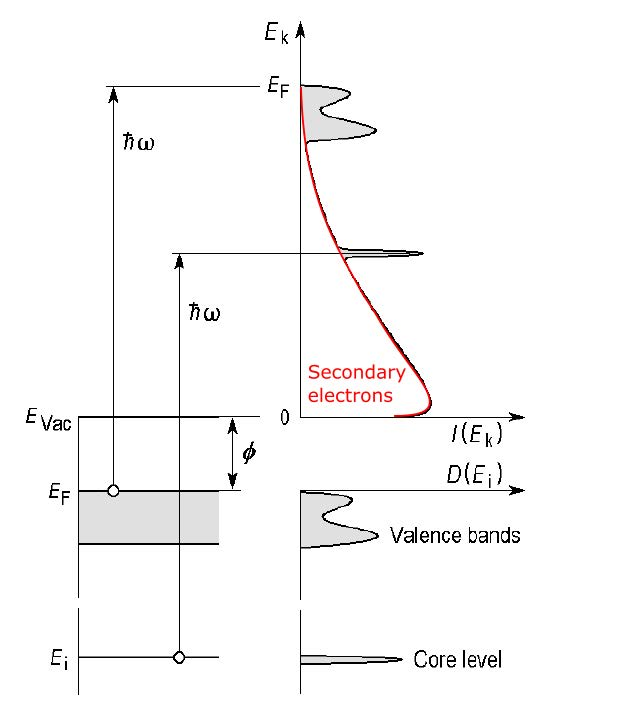
\includegraphics[width=0.5\textwidth]{EDC_DJ.jpg}
            \caption{Entstehung der EDC für den Valenzbandbereich und die Kernniveaus.
            Kopiert aus \cite{oura_surface_2003}.}
            \label{fig:EDC}
        \end{figure}
        Wird die Anzahl detektierter Elektronen gegen ihre kinetische Energie aufgetragen, ergibt sich die Energieverteilungsfunktion (\textit{energy distribution curve}, EDC).
        Diese spiegelt die Zustandsdichte der entsprechenden Probe wider, was in \autoref{fig:EDC} dargestellt ist.        
        Links im Bild ist die elektronische Struktur in einem Festkörper zu sehen, rechts die zugehörige Energieverteilungskurve.
        Hierbei lässt sich diese in zwei Bereiche teilen, den der Valenzelektronen bei hohen kinetischen Energien und der Kernniveauelektronen bei niedrigen kinetischen Energien.
        Energetisch sind diese Bereiche durch die unterschiedlichen Bindungsstärken separiert, wobei die Kernniveauelektronen stark gebunden sind und damit eine höhere Photonenenergie erfordern.
        Sie unterscheiden sich ebenfalls durch ihre Breite, wobei die Kernniveaus aufgrund ihrer starken Lokalisierung scharfe Signale zeigen und die Valenzbänder aufgrund der Dispersion der Bänder eher breite Strukturen~\cite{Hüfner}.

        Um beide Anteile im oberflächensensitiven Bereich zu untersuchen sind dabei verschiedene Photonenenergien von Nöten um Elektronen mit entsprechender kinetischer Energie auszulösen.
        Der Valenzbandbereich nahe der Fermikante lässt sich mittels der ultravioletten Strahlung genauer untersuchen, was in \autoref{sec:UPS} genauer erläutert wird.
        Zur Untersuchung der kernnahen Zustände wird Röntgenstrahlung (\textit{X-Ray}) eingesetzt und genauer in \autoref{sec:XPS} erläutert.
        Der Prozess der Photoelektronenemission kann für beide Energiebereiche durch das drei Stufenmodell beschrieben werden, wodurch auch die unterschiedlichen Photonenenergien begründet werden können.
        Diese Modell wird in \autoref{sec:3Stufen} eingeführt.

        \subsection{Drei Stufenmodell} \label{sec:3Stufen}
        \begin{figure}
            \centering
            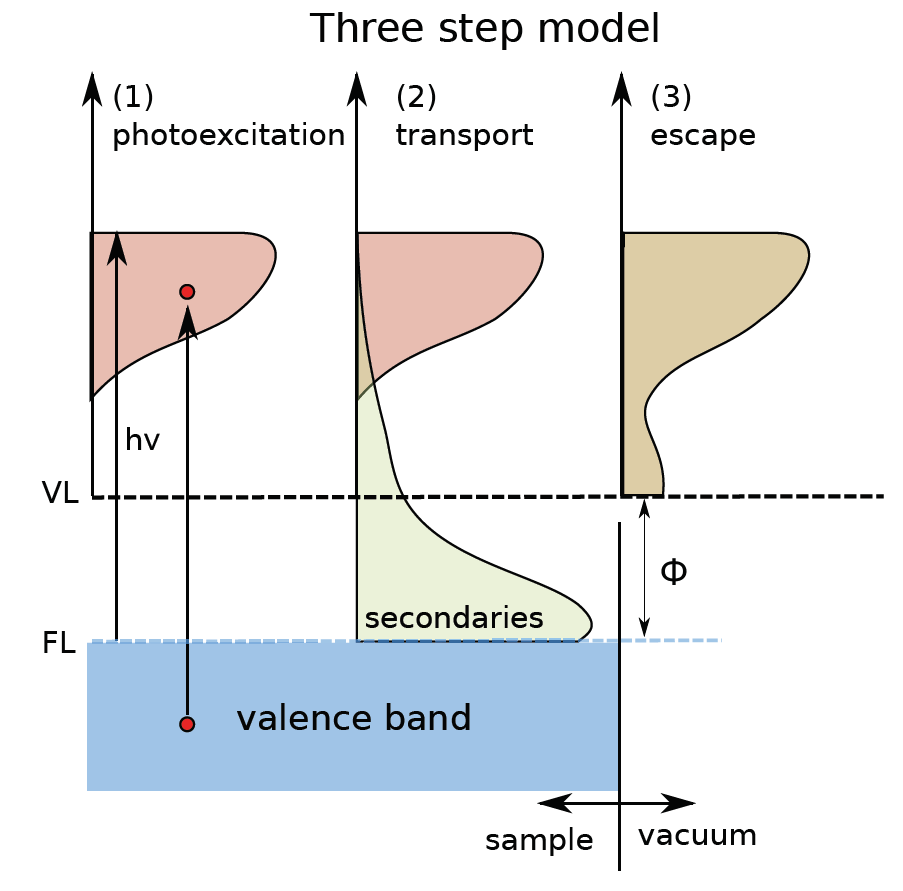
\includegraphics[width=0.5\textwidth]{3Stufen}
            \caption{Das drei Stufenmodell für die Photoelektronenemission.
            Bestehend aus (1) Absorption, (2) Transport zur Oberfläche und (3) Austritt aus der Oberfläche.
            Kopiert und modifiziert aus~\cite{zhang_synchrotron_2018}.}
            \label{fig:3Stufen}
        \end{figure}
        \begin{figure}
            \centering
            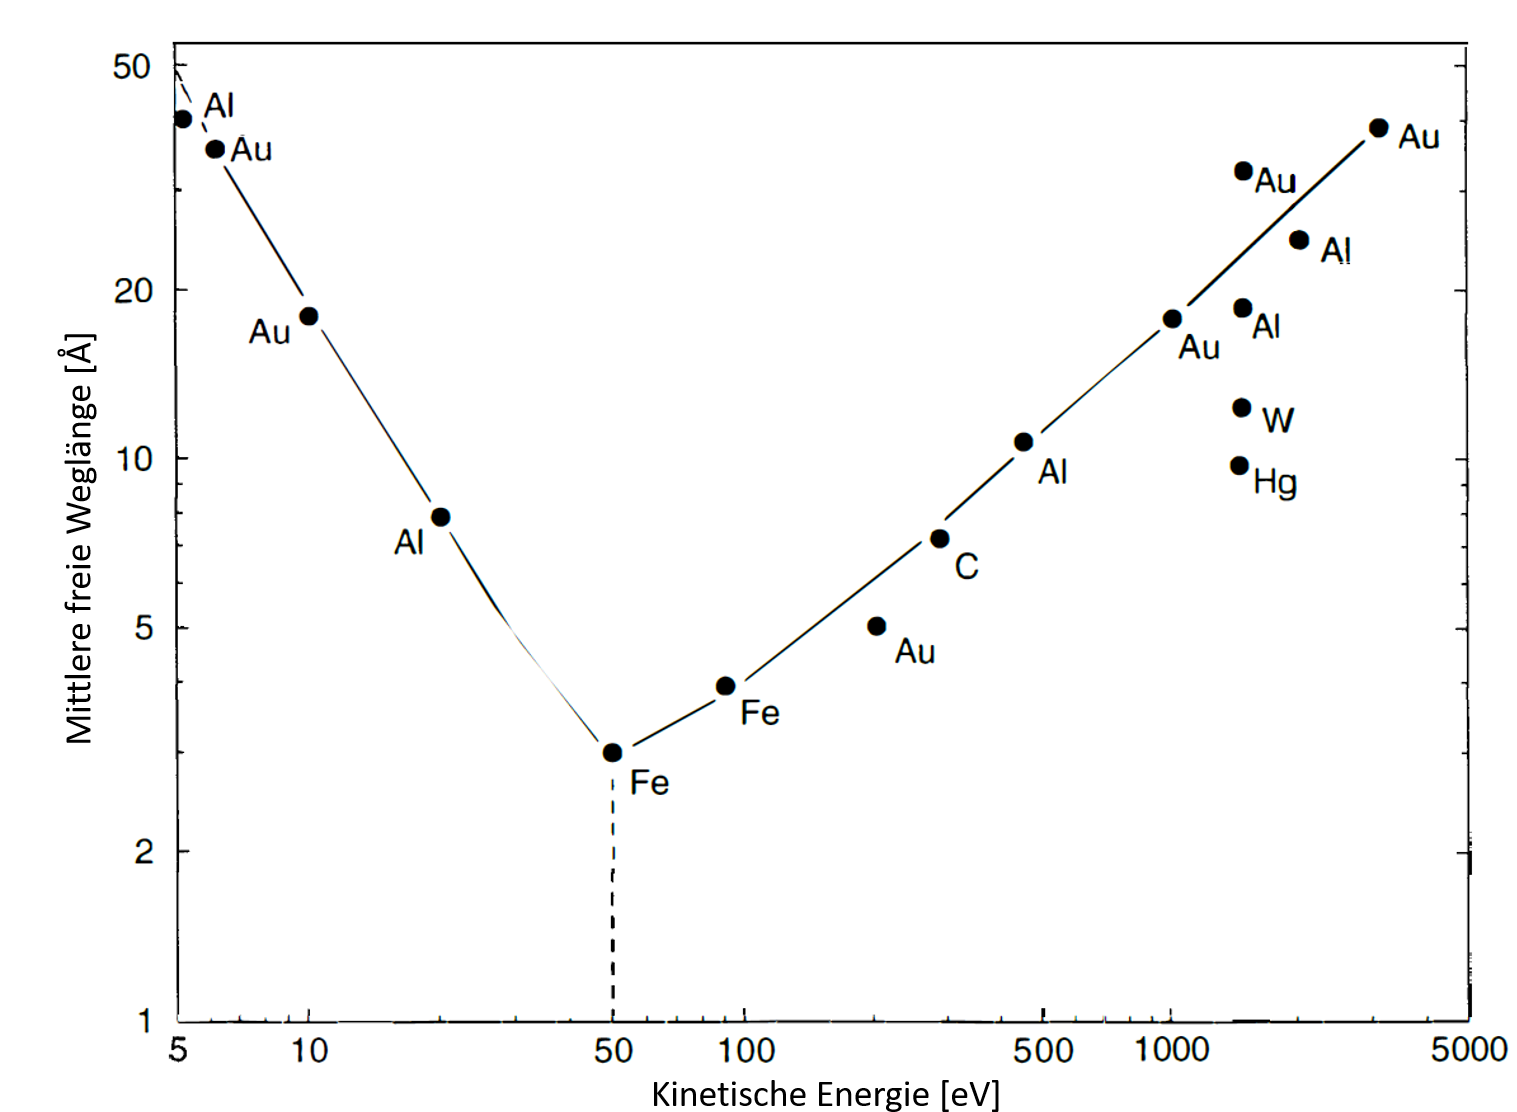
\includegraphics[width=0.6\textwidth]{Weg2.png}
            \caption{Inelastische mittlere freie Weglänge für Elektronen in verschiedenen Materialien. Aus~\cite{Hüfner} und bearbeitet.}
            \label{fig:Weg}
        \end{figure}
        Der Prozess der Photoelektronenemission lässt sich in einem Model mit drei unabhängigen Stufen erklären.
        Das Model ist in \autoref{fig:3Stufen} schematisch zu sehen.
        Der erste Schritt ist die Absorption des Photons, wodurch das Elektron aus seiner Bindung gelöst wird und in einen unbesetzten Zustand angeregt wird.
        Dabei besitzt das Elektron eine gewisse kinetische Energie mit der es innerhalb des Festkörpers zur Probenoberfläche wandert.
        Auf dem Weg zur Oberfläche können die Elektronen Stößen unterfahren, wodurch es im Fall eines elastischen Stoßes mit anderen Elektronen Energie und damit Informationen über deren Ursprung verlieren.
        Die gestreuten Elektronen, sogenannte Sekundärelektronen, erzeugen einen kontinuierlichen Untergrund und ihr Beitrag steigt mit abnehmender kinetischer Energie an.
        Die mittlere freie Weglänge, die ein Elektron im Festkörper zurücklegt ohne inelastische zu streuen, ist stark abhängig von der kinetischen Energie, wie in \autoref{fig:Weg} gezeigt ist.
        Es ist zu erkennen, dass Elektronen mit einer kinetischen Energie im Bereich von \SIrange{30}{100}{\electronvolt} und nicht inelastisch gestreut wurden, aus einer Tiefe von nicht mehr als \SI{5}{\angstrom} herrühren und somit aus dem oberflächennahen Bereich.
        Ist die kinetische Energie des Elektrons größer als die Austrittsarbeit der Probe, so kann das Elektron die Oberfläche in einem dritten Schritt verlassen.
        An der Oberfläche des Festkörpers ist die Periodizität gebrochen, wodurch das Elektron gebeugt wird und die senkrechte Komponente des Impulsvektors nicht erhalten bleibt.
        Dahingegen bleibt der Impulsvektor parallel zur Oberfläche $\vec{k}_{||}$ erhalten.
        Dies wird sich bei der winkelaufgelösten Photoelektronenspektroskopie in \autoref{sec:ARPES} zu Nutzen gemacht.

        Die Wahrscheinlichkeit für einen Übergang aus dem Anfangszustand $\Psi_\text{i}$ (i = \textit{intinal}) in einen Endzustand $\Psi_\text{f}$ (f = \textit{final}) wird durch Fermis goldene Regel beschrieben.
        Damit ist die Intensität des Photoemissionsprozesses 
        \begin{equation}
            I_\text{fi} \propto \frac{2\pi}{\hbar} \abs{\bigl<\Psi_\text{f}|\Delta|\Psi_\text{i}\bigr>}^2 \, \delta\left(E_\text{f}-E_\text{i}-h\nu\right)
            \label{eqn:Fermi_gold}
        \end{equation}
        abhängig von der verwendeten Photonenenergie $h \nu$, sowie der Energie des Anfangszustandes $E_\text{i}$ und Endzustandes $E_\text{f}$.
        Hierbei stellt $\Delta \approx \frac{\symup{e}\hbar}{m}\vec{A}\cdot\vec{p}$ einen Operator dar und beschreibt die Interaktion zwischen dem äußeren Feld (klassische Vektorpotential des externen elektrischen Feldes $\vec{A}$) und dem austretenden Elektron~\cite{cao_theory_2010}.
        Bei den Übergängen die durch das Photon angeregt werden, handelt es sich um direkte Übergänge und damit um einen Impuls ($\vec{k}$) erhaltenen Prozess.
        Der Wellenvektor des Endzustandes $\vec{k}_\text{f}$ unterscheidet sich nur um einen reziproken Gittervektor $\vec{G}$ vom Wellenvektor des Anfangszustands $\vec{k}_\text{i}$.
        Ob ein Übergang nun erlaubt ist oder nicht wird also durch die Symmetrien des Anfangs- und Endzustands bestimmt.
        Zudem ist die Polarisation des einfallenden Photons entscheidend.
        Die $\delta$-Funktion berücksichtigt das Prinzip der Energieerhaltung.
        Um Elektronen mittels Photoelektronenspektroskopie zu detektieren, muss der Endzustand oberhalb der Vakuumenergie liegen.

        % Lokale Effekte vernachlässigt, N Elektronen im Anfangszustand
        Ein weiteres Model zur Beschreibung der theoretischen Photoelektronenemission ist das ein Stufenmodell.
        Diese fasst alle drei Elemente des drei Stufenmodell zu einem zusammen, wobei der Endzustand durch einen Zustand beschrieben wird, der sich im Vakuum frei ausbilden kann, aber in Richtung der Oberfläche gedämpft wird.
        Das ein Stufenmodell behandelt den Prozess der Photoemission als einen kohärenten Prozess eines Mehrteilchenproblems.
        Zusätzlich berücksichtigt das Modell, dass sich der Grundzustand vom Endzustand durch die Anregung und Erzeugung eines Lochs unterscheidet.

        \subsection{Röntgenphotoelektronenspektroskopie - XPS} \label{sec:XPS}
            Um die Kernniveaus des Systems zu betrachten, wird weiche Röntgenstrahlung mit einer Energie von \SIrange{0.1}{10}{\kilo\electronvolt} verwendet~\cite{Fauster} und wird mit XPS (\textit{X-Ray Photoelectronspectroscopy} abgekürzt.
            Diese Energien sind nur mit klassischen Röntgenquellen oder einem Synchrotron erreichbar.
            Mit dieser Methode lässt sich die chemische Zusammensetzung der Probe untersuchen, da die typischen Bindungsenergien größer als \SI{50}{\electronvolt} sind und damit nicht direkt an Bindungen beteiligt sind.
            Leicht unterschiedliche Positionen in der Bindungsenergie für verschiedene Ionisationszustände und Bindungszustände (z.B. Oberflächenatome oder tieferliegende Atome) können dabei Rückschlüsse auf die chemische Umgebung zulassen.
            Auf Grund der Symmetrien der Wellenfunktion der Kernniveaus ist ihre Bindungsenergie unabhängig vom Impulsvektor und das Signal zeigt die Form einer Lorentz-Funktion~\cite{Hüfner}.
            Maßgeblich wird die Halbwertsbreite des Signals durch das inverse der Lebenszeit des entsprechenden Zustands bestimmt, was die Halbwertsbreite der Lorentz-Funktion bestimmt.

            Bei experimentellen Daten ergeben sich verschiedene verbreiternde Effekte, die durch die Faltung mit einer Gaußfunktion berücksichtigt werden können.
            So fließt die Energieauflösung des Detektors mit in die gemessene Halbwertsbreite ein, welches die ermittelte kinetische Energie beeinflusst.
            Die Halbwertsbreite der verwendeten Photonenenergie sorgt für unterschiedliche kinetische Energien der vom gleichen Zustand emittierten Elektronen.
            Durch Vermessen des Systems bei niedrigen Temperaturen kann eine Verbreiterung des Signals auf Grund von der Reduktion thermischer Effekte vermindert werden.
            Vermehrt treten bei Metallen einseitige Verbreiterungen auf, welche auf die Wechselwirkung zwischen dem Valenzband und dem im Kernniveau erzeugten Loch zurückzuführen ist.
            Dieses zusätzliche positive Potential führt zu einer Verschiebung zu größeren Bindungsenergien.
            Ebenso kann eine mehrfache Ionisation durch Multiphotonenabsorption oder interne Prozesse wie den Augerprozess zu Energieverschiebungen der emittierenden Zustände und damit einer Asymmetrie führen.
            % inelastische Streuungen der Photoelektronen zurückzuführen ist. - Asymmetrie?
            % \textbf{???} Die Linien erfahren eine weiter Verbreiterungen, wenn sich durch die Spin-Bahn-Kopplung Dubletts ausbilden und nur eine geringe Energieaufspaltung zeigen.
            % Diese Aufspaltung resultiert aus der Wechselwirkung zwischen dem Spin des Valenzbandes und des photoionisierten Kernniveaus, was nun auch einen Spin trägt.
        % \subsection{Röntgenabsorptionspektroskopie - XAS}
        %     Für die Durchfürung von Röntgenabsorptionsmessungen ist eine durchstimmbare Photonenquelle im weichen Röntgenbereich notwendig.
        %     Dies ist aktuell nur durch Synchrotrons und Freieelektronenlaser realisierbar.
        %     Hierbei wird die Photonenenergie $h\nu$ über einen bestimmten Bereich variiert. % in der eine Abosrptionskante liegt abgetastet.
        %     Trifft ein Photon auf die Oberfläche so wird dieses absorbiert und kann ein Photoelektron auslösen.
        %     Wie viele Photonen diesen Prozess anregen können hängt davon ab, ob sich Elektronen bei der Energie $h\nu = E_\text{B}+\phi$ befinden.
        %     Energien an den schlagartig die Absorption steigt werden auch Absorptionskanten genannt und sind charakteristisch für verschiedene Elemente. 
        %     Es handelt sich dabei dann um einen Übergang aus einem bestimmten Kern nahen Zustand in einen unbestzten Zustand.
        %     Durch die Wahl der Polarisation des Lichtes kann auch spinsensetiv selktiert werden, welche Elektronen ausgelöst werden.

        \subsection{Ultraviolettphotoelektronenspektroskopie - UPS} \label{sec:UPS}
            Das Valenz- und Leitungsband kann mit ultravioletter Strahlung im Bereich von \SIrange{10}{100}{\electronvolt} untersucht werden und wrd als Ultraviolettphotoelektronenspektroskopie bezeichnet (UPS, \textit{Ultraviolett Photoelectronspectroscopy}~\cite{Fauster}.
            Photonen in diesem Energiebereich können in Laboren mit Gasentladungslampen erzeugt werden, sind aber ebenfalls an einem Synchrotron verfügbar.
            Die zuvor gering gebundenen Elektronen besitzen in Folge dessen eine kinetische Energie, die im oberflächensensitiven Bereich liegt.
            Zusätzlich ist durch die niedrige Photonenenergie die Wechselwirkungswahrscheinlichkeit mit den entsprechenden Zuständen groß, sodass möglichst viele Elektronen emittiert werden.
            % In diesem Energiebereich wird ebenfalls die Photoemissionsorbitaltomographie genutzt, welche in \autoref{sec:MOT} eingeführt wird.
            % Auf Grund der starken $\vec{k}$-Abhängigkeit im Valenzband und dessen Erhaltung sowie der niedrigen Photonenenergien können bei der Ultraviolettphotoelektronenspektroskopie einige Zustände nicht abgebildet werden~\cite{Hüfner}.
            % Bei XPS hingegen ist dies kaum eingeschränkt, denn durch die hohen Energien kann die ganze Brillouinzone als Akzeptanzbereich genutzt werden~\cite{Hüfner}.

        \subsection{Winkelaufgelöste Photoelektronenspektroskopie - ARPES} \label{sec:ARPES}
            Durch die Erfassung der Austrittswinkel der emittierten Elektronen können Rückschlüsse auf die Bandstruktur innerhalb der Probe gezogen werden.
            Hierzu wird vom Analysator nur ein gewisser Winkelbereich entlang einer Richtung ($k_\text{x}/k_\text{y}$) akzeptiert.
            Durch Variation der Winkel zwischen Probe und Analysator wird ein kleinere Teilbereiche von $k_\text{||} = \sqrt{k_\text{x}^2 + k_\text{y}^2}$ erfasst.
            \begin{figure}
                \centering
                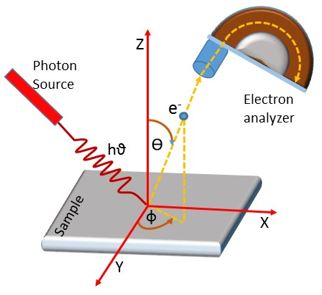
\includegraphics[height=5cm]{ARPES.jpg}
                \caption{Versuchsanordnung zur Messung von winkelaufgelösten Photoemissionspektren. Kopiert aus \cite{ARPES}.}
                \label{fig:ARPES}
            \end{figure}
            Schematisch ist dies in \autoref{fig:ARPES} dargestellt.
            Für jede Winkelkombination aus polarem $\theta$ und azimutalen $\phi$ Winkel wird ein UPS-Spektrum aufgezeichnet.
            Die entsprechenden Impulsvektoren der Elektronen lassen sich aus den Winkeln und der kinetischen Energie nach
            \begin{gather}
                k_\text{x} = \sqrt{\frac{2 \text{m}_\text{e} E_\text{Kin}}{\hbar^2}} \sin\theta \cos\phi \\
                k_\text{y} = \sqrt{\frac{2 \text{m}_\text{e} E_\text{Kin}}{\hbar^2}} \sin\theta \sin\phi
            \end{gather}
            berechnen~\cite{MM_4}.
            So ergibt sich aus den energieselektierten Elektronen ein Teilbereich der Bandstruktur $E(k_\text{||})$.
            
            % Durch die Korrelation zwischen dem Impuls und der kinetischen Energie
            % \begin{equation}
            %     E_\text{Kin} = \frac{\hbar^2 \vec{k}^2}{2 m_\text{e}}
            % \end{equation}
            % über das reduzierte planksche Wirkungsquantum $\hbar$ und der Elektronenmasse $m_\text{e}$
            % 
            % Im ein Stufen Model ergibt sich
            Unter Berücksichtigung der Austrittswinkel der Elektronen, sowie des finalen Zustands $\Psi_\text{f}$ mit einer Energie $E_\text{Kin}$, ergibt sich die Photoelektronenintensität in entsprechende Richtung
            \begin{equation}
                I(\theta, \phi, E_\text{Kin}) \propto \sum_i \abs*{\bigl<\Psi_\text{f}(\theta, \phi, E_\text{Kin})|\vec{A}\cdot\vec{p}|\Psi_\text{i}\bigr>}^2 \times \delta\left(E_\text{i}+E_\text{Kin}+\Phi-h\nu\right))
                \label{eqn:ARPES}
            \end{equation}
            vom Anfangszustand $\Psi_\text{i}$ in der Dipolapproximation~\cite{MM_2}.
            Dabei tragen alle erlaubten Übergänge aus den besetzten Anfangsstadien $i$ zur Gesamtintensität bei.

    \section{Photoelektronenemissionsmikroskopie} \label{sec:PEEM}
        Die Photoelektronenemissionsmikroskopie vereinigt spektroskopische und mikroskopische Methoden. % ist eine sehr viel versprechende Technik, die für immer mehr Aufsehen in den letzten Jahren gesorgt hat.
        Sie nutzt die Prinzipien der Energie- und Impulserhaltung, um Bilder der Proben im Realraum oder Impulsraum aufzulösen.
        Zuerst wurde dies 1933 durch E. Brüche entdeckt, der eine Realraumaufnahme einer Zinkplatte mit Hilfe von Photoelektronen und einer magnetischen Linse auf einem Leuchtschirm abbildete~\cite{bruche_elektronenmikroskopische_1933}.
        
        \begin{figure}
            \centering
            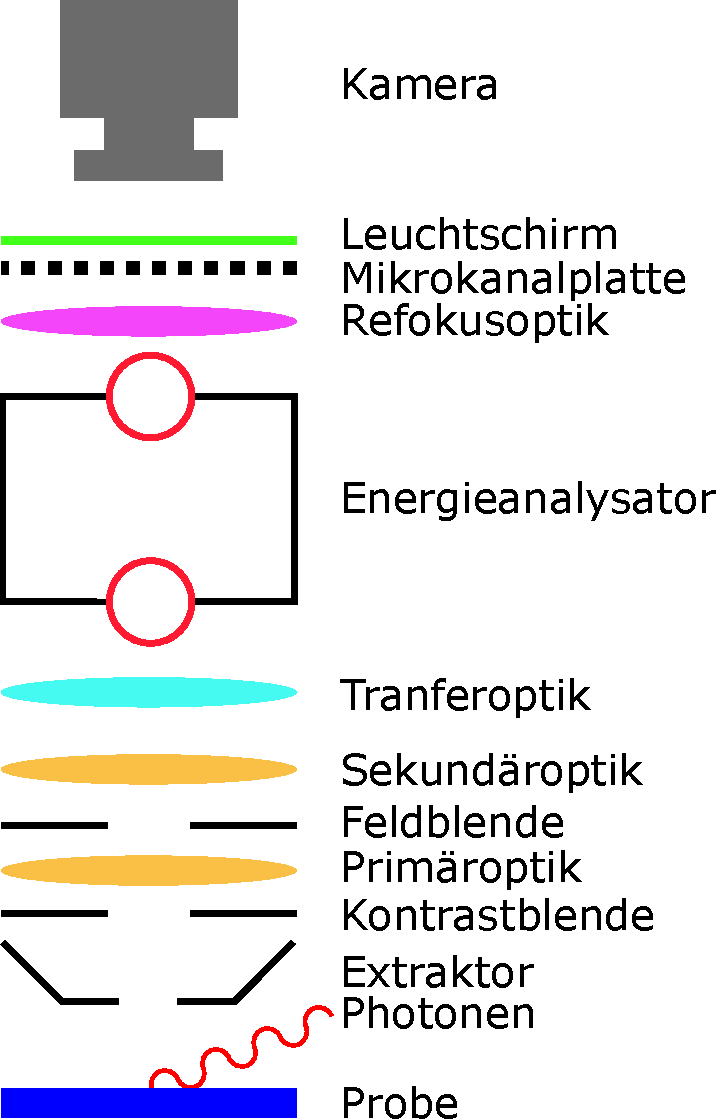
\includegraphics[width=0.4\textwidth]{PEEM_new_Valentin.pdf}
            \caption{Vereinfachter Aufbau eines 2D Photoelektronenmikroskops.} 
            % Vorlage aus~\cite{KUCH}, modifiziert. - PEEM_schemaneu.png}
            \label{fig:MM}
        \end{figure}
        Ein exemplarischer Aufbau ist in \autoref{fig:MM} zu sehen.
        Die durch die Photonen, aus einem Energiebereich von \SIrange{10}{100}{\electronvolt}, angeregten Elektronen werden durch ein starkes elektrisches Feld von einigen \si{\kilo\volt} von der Probe zum Analysator hin beschleunigt.
        Durch diese große Spannung zwischen Probe und Extraktor ist es möglich, einen großen Sichtbereich im Impulsraum abzudecken.
        % Dies ist nötig, da durch den streifenden Einfall der Photonen und der Abberation der elektrostatischen Linsen nur einen kleinen Akzeptanzwinkel zur Verfügung stehen würde.
        Wichtig bei dem Extraktorfeld ist, dass das Feld zwischen Probe und Extraktor sehr homogen ist, damit der Austrittswinkel erhalten bleibt.
        Dies hat zur Folge, dass die Probe eine möglichst ebene Oberfläche aufweisen muss.
        % Anschließend werden die Elektronen durch elektrostatische Linsen fokussiert und mittels elektrostatischer Verschiebungslinsen zentriert.
        Anschließend treffen die Elektronen in der hinteren Brennebene auf die Kontrastblende mit der die Winkelakzeptanz der Austrittswinkel definiert wird.
        Mit Hilfe der Primäroptik werden die Elektronen fokussiert, sodass sich in der Bildebene das Realraumbild ergibt.
        Um das Bild ins Zentrum der hier befindenen Feldblende/Iris zu fokussuieren, stehen zusätzlich elektrostatische Verschiebungslinsen zur Verfügung.
        Mit der Feldblende wird ein Ausschnitt auf der Probe ausgewählt, von der die emittierten Elektronen erfasst werden.

        Im Anschluss an das erste Linsensystem folgt ein weiters Linsensystem aus elektrostatischen Linsen, die das Realraumbild auf den Ausgang des Linsensystems fokussieren.
        % Dieses Linsensystem ist zur Korrektur von Aberrationen und zur Ausrichtung des Bildes verantwortlich.
        % Hierfür stehen ebenso zwei magnetische Verschiebungslinsen zur Verfügung, um eine Verschiebung des Elektronenbündels zu korrigieren.
        Hier gehen die Elektronen in ein Transferlinsensystem über, welches dafür sorgt, dass ein identisches Abbild auf die Eingangsblende des Analysators trifft.
        Mit Hilfe des Transferlinsensystems wird festgelegt, ob ein Bild des Real- oder Impulsraums auf die Eingangsblende abgebildet wird.
        Als Energieanalysator kommt ein hemisphärischer Analysator zum Einsatz.
        Beim hemisphärischen Analysator werden die Elektronen zwischen zwei Halbkugeln durch ein statisches elektrisches Feld auf eine Kreisbahn gezwungen.
        Dabei erreichen nur Elektronen in einem kleinen Bereich um die eingestellte Pass-Energie $E_\text{Pass}$ die Ausgangsblende.
        
        Nach dem Detektor gibt es eine weiter Linseneinheit, welche zusammen mit einer Blende das gewünschte energieaufgelöste Bild auswählt und es auf die Detektorgröße aufweitet.
        Je kleiner die Blende gewählt wird, desto besser ist die Energieauflösung, aber desto kleiner die Gesamtintensität.
        Anschließend durchlaufen die Elektronen eine Mikrokanalplatte und treffen auf den Phosphorschirm, der infolgedessen an diesen Auftrittsstellen aufleuchtet.
        Durch die CMOS (\textit{Complemantary metal-oxid-semiconductor}) Kamera wird dieses Leuchten registriert und das räumliche oder rekursive Bild kann rekonstruiert werden~\cite{SPECS-MM}.
        % Bei dem Detektor handelt es sich um eine CMOS Kamera die das Bild der auf den Leuchtschirm auftreffenden Elektronen aufnimmt.
        % CCD (\textit{Charge Coupled Device}) Detektoren sind ein Standard bei ARPES Messungen, sie integrieren die analoge Photonenintensitäten oder einzelne Lichtblitze werden aufgezeichnet.
        % Einer der Nachteile ist die geringe Abtastrate auf Grund der hohen Erholungszeit.
        % Hier wird allerdings eine CMOS (\textit{Complemantary metal-oxid-semiconductor}) Kamera verwendet.
        % Dabei wird ein einzelnes Bild in nur wenigen Millisekunden erfasst, dies ist durch die Kombination von Kamera und Grafigprozessor möglich.
        % Der Vorteil der CMOS Kamera Technik gegenüber der klassischen CCD  Kamera Technik ist, die Erfassung der wahren Pulszählraten~\cite{CMOS}.
        
        Das Photoelektronenemissionsmikroskop kann in zwei verschiedene Betriebsmodi betrieben werden, der Realraum- oder Impulsraumaufnahme.
        \begin{figure}
            \centering
            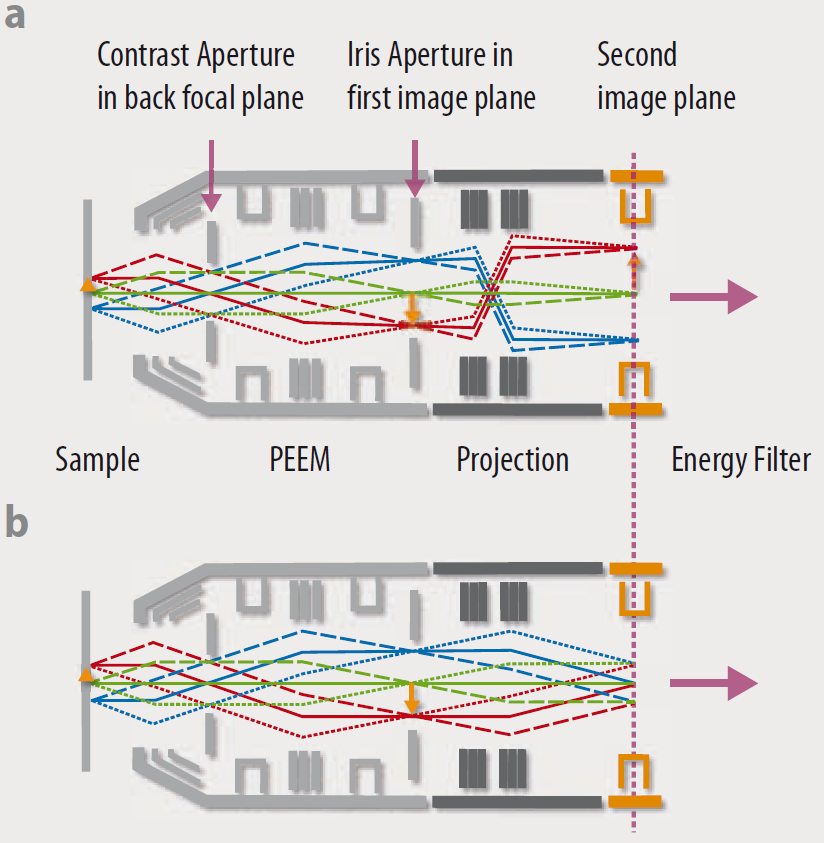
\includegraphics[width=0.5\textwidth]{Real_k.PNG}
            \caption{Verschiedene Konfigurationen der Transferlinse, um zwischen Realraum und Impulsraum Bild umschalten zu können.
            (a) bildet die Transferlinse das Realraumbild auf die Eintrittsblende des Analysators ab, wodurch sich die Aufnahme des Realraums ergibt.
            (b) es ergibt sich das Bild im reziproken Raum und die Transferlinse bildet das Beugungsbild auf die Eintrittsblende ab.
            Aus~\cite{Focus}.}
            \label{fig:real_k}
        \end{figure}
        Für den Realraum ist dies in \autoref{fig:real_k}\,a und für den Impulsraum in \autoref{fig:real_k}\,b dargestellt.
        Im vorderen Teil, dem PEEM (\textit{Photon emitted electron microscopy}), ändert sich nichts wohingegen die Transferlinse dafür sorgt, dass etweder das Beugungs- oder Realraumbild auf die Eintrittsblende des Analysators abgebildet wird.
        Vorteil der Umschaltung zwischen den Modis ist, dass auf sehr kleinen Bereichen die sich im Realraum bestimmt wurden Messungen im reziproken Raum durchführen lassen~\cite{suga_photoelectron_2021}.
        Realisiert wird dies durch die Transferlinse, die durch eine entsprechende Fokussierung das Bild generiert.
        Dies ist nur möglich, wenn die gesamte Ausrichtung passt und sich das Realraumbild immer an der Stelle der Bildebene ergibt und das Beugungsbild in der hinteren Brennebene.
        

        \subsection{Impulsraumaufnahmen}
            Mit Hilfe des Linsensystems wird gewährleistet, dass auf die Eintrittsblende des Analysators das Beugungsbild aus der hinteren Brennebene abgebildet wird.
            Außerdem bleibt bei der Aufnahme im Impulsraum durch die gesamte Abbildungsoptik der Austrittswinkel erhalten.
            Das verwendete Mikroskop kann für eine kinetische Energie kleiner als \SI{50}{\electronvolt} einen Austrittswinkel von bis zu $\pm\SI{90}{\degree}$ erfassen~\cite{SPECS-MM}.
            Für größere kinetische Energien wird das Sichtfeld auf $\pm\SI[per-mode=reciprocal]{3.6}{\per\angstrom}$ beschränkt~\cite{SPECS-MM}.
            Allerdings kann mit der Kontrastblende der aufgenommene Winkelbereich eingeschränkt werden.
            Dabei spielt es keine Rolle, wo die Elektronen im durch die Feldblende ausgewählten Bereich emittiert werden.

            Dies wird als Impulsmikroskopie (\textit{Momentum Microscopy}) bezeichnet.
            Bei der Impulsmikroskopie ist die zeitgleiche Erfassung des polaren und azimutalen Austrittswinkel von großer Bedeutung. 
            So entsteht durch die zusätzliche Sortierung der Elektronen nach ihrer kinetischen Energie ein dreidimensionaler Datensatz, woraus sich die Bandstruktur extrahieren lässt.

        \subsection{Realraumaufnahmen}
            Gleichzeitig sind Aufnahmen im Realraum möglich und auf dem Eintrittsspalt des Energieanalysators wird das Bild der Oberfläche projiziert (siehe \autoref{fig:real_k}\,a).
            Das Bild wird bei festen Energiefilter-Einstellungen aufgenommen, wodurch der Modus als PEEM bezeichnet wird.
            Bei einem Blendendurchmesser der Feldblende von \SI{20}{\micro\meter} und der Vergrößerung von~\num{5} beläuft sich der ausgewählten Bereich auf ein Größe von \SI{4}{\micro\meter}~\cite{SPECS-MM}.
            Eine Verbesserung des Auflösungsvermögens kann durch Verringerung des Durchmessers der Kontrastblende erzielt werden.
            Mit Hilfe der Kontrastblenden kann eine laterale Auflösung von einigen \si{\nano\meter} erreicht werden~\cite{locatelli_chemical_2015}. 

            Durch unterschiedliche Austrittsarbeiten innerhalb der Oberfläche kann mit dieser Technik die Homogenität der Probe untersucht werden.
            Hierdurch ergeben sich Bereiche unterschiedlicher Intensität, was durch den Kontrast erkennbar ist.
            Bei Verwendung von zwei unterschiedlichen Polarisationen kann die magnetische Domänenbildung sichtbar gemacht werden.
            Dabei werden meist zirkular polarisierte Photonen eingesetzt, was als Intensitätsinvertierung sichtbar wird.
        
    \section{Photoemissionsorbitaltomographie} \label{sec:MOT}
        Zur Identifizierung von Molekülorbitalen vereinen sich in der Photoemissionsorbitaltomographie die experimentelle Impulsmikroskopie und die theoretische Vorhersage über die Photoelektronenintensität.
        Durch gezielte Annahmen kann dabei aus den Übergangswahrscheinlichkeiten ein theoretisch berechnetes Bild im Impulsraum rekonstruiert werden.
        Dieses kann nunmehr mit den gemessenen impulsaufgelösten Bildern verglichen werden, wenn sich die Molekülorbitale regelmäßig und langreichweitig zueinander ausrichten.
        Grund hierfür ist der im Vergleich zur Dispersion größerer Energieabstand der Molekülorbitale, wodurch eine eindeutige Zuordnung ermöglicht wird~\cite{puschnig_reconstruction_2009}.

        \begin{figure}
            \centering
            \begin{subfigure}{0.3\textwidth}
                \centering
                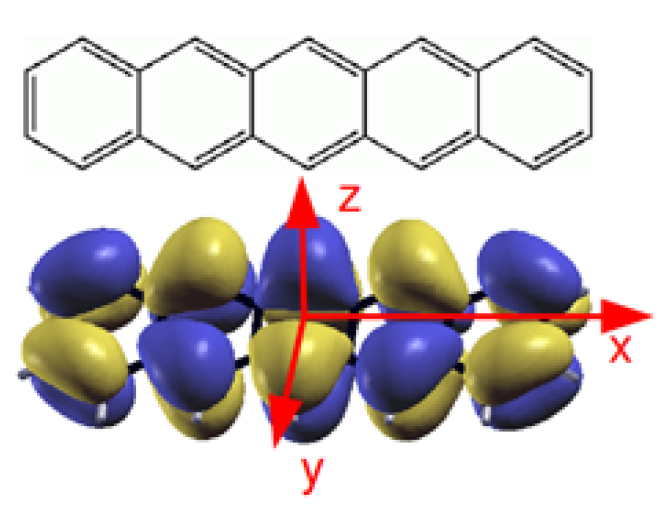
\includegraphics[width=0.9\textwidth]{DFT1.PNG}
                \caption{}
                \label{fig:DFT1}
            \end{subfigure}
            \begin{subfigure}{0.3\textwidth}
                \centering
                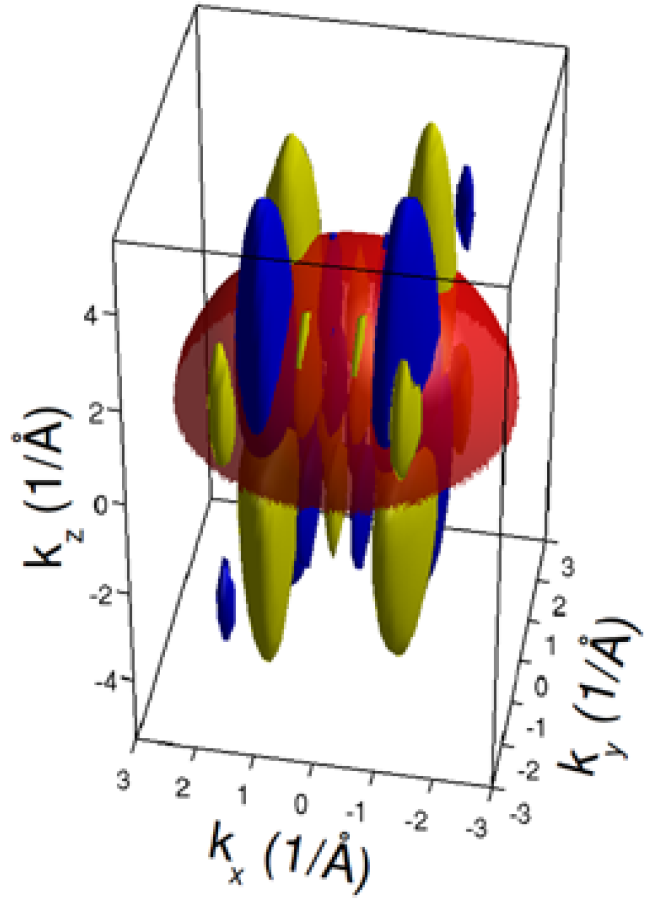
\includegraphics[width=0.9\textwidth]{DFT2.PNG}
                \caption{}
                \label{fig:DFT2}
            \end{subfigure}
            \begin{subfigure}{0.3\textwidth}
                \centering
                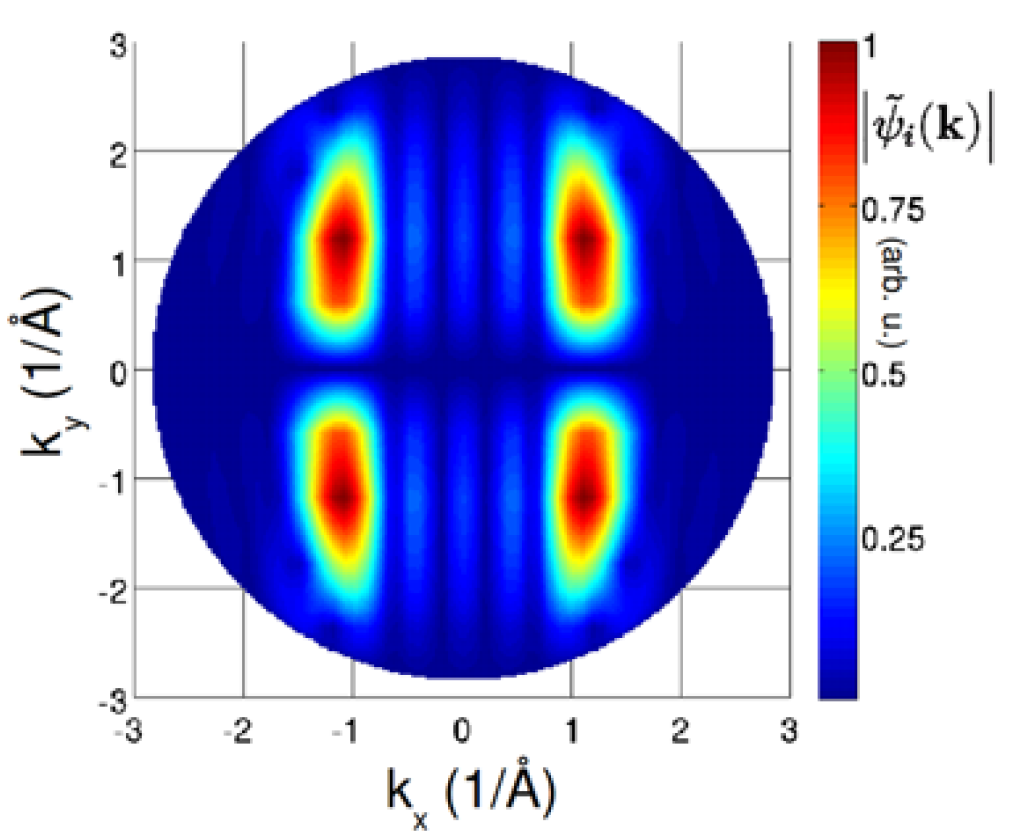
\includegraphics[width=0.9\textwidth]{DFT3.PNG}
                \caption{}
                \label{fig:DFT3}
            \end{subfigure}
            \caption{In (\subref{fig:DFT1}) ist die sich aus der Dichtefunktionaltheorie (DFT) ergebene Struktur von Pentacen gezeigt.
            Die durch Fouriertransformation gewonnen Orbitalstruktur im reziproken Raum (\subref{fig:DFT2}).
            (\subref{fig:DFT3}) die Projektion der Fouriertransformation der Molekülorbitale für eine feste kinetische Energie.
            Aus~\cite{MM_2}}
            \label{fig:DFT}
        \end{figure}
        Um eine theoretische Vorhersage für Molekülorbitale treffen zu können, müssen drei Punkte erfüllt werden.
        Dabei muss gelten, dass
        \begin{enumerate}
            \item die Emission von $\pi$-Orbitalen großer Moleküle herrührt,
            \item der Winkel zwischen Polarisationsvektor $\vec{A}$ und Richtung der austretenden Elektronen $\vec{k}$ klein ist und
            \item die Moleküle aus leichten Atomen bestehen.
        \end{enumerate}
        Hierdurch kann die Näherung von ebenen Wellen akzeptiert werden~\cite{MM_2}.
        Durch die Approximation des Endzustands als ebene Wellen ist der Photoelektronenstrom proportional zur Fouriertransformation des Anfangszustandes $\tilde{\Psi}_\text{i}(\vec{k})$.
        So geht die Photoelektronenintensität aus \autoref{eqn:ARPES} in
        \begin{equation}
            I_\text{i}(\theta, \phi) \propto \frac{\abs*{\tilde{\Psi}_\text{i}(\vec{k})}^2}{\abs*{\vec{A}\cdot\vec{k}}^2}
        \end{equation}
        über.
        Mit dem Polarisationsfaktor $\abs*{\vec{A}\cdot\vec{k}}$, der den Winkel zwischen einfallenden Photonen und austretenden Elektronen berücksichtigt, der durch die experimentelle Geometrie gegeben wird.
        Somit ist die Intensität im Impulsraumbild lediglich abhängig von der Dichte im Anfangszustand. % azimuntalen und polaren Winkel, also folglich $k_\text{x}$, $k_\text{y}$ und der kinetischen Energie der Elektronen, sowie der Dichte im Anfangszustand.

        Unter Zuhilfenahme der Dichtefunktionaltheorie (DFT) kann die Struktur der beteiligten Moleküle im Realraum berechnet werden~\cite{database}.
        Dies ist beispielhaft in \autoref{fig:DFT1} für Pentacen dargestellt.
        Die Orbitalstruktur beziehungsweise die Aufenthaltswahrscheinlichkeiten der Elektronen abhängig von ihrem Impuls ergibt sich mittels der Fouriertransformation (siehe \autoref{fig:DFT2}).
        Schließlich wird die Fouriertransformation entlang einer Ebene konstanter kinetischer Energie geschnitten, was der roten Hemisphäre in \autoref{fig:DFT2} entspricht.
        Die daraus resultierende Projektion in \autoref{fig:DFT3}~\cite{brandstetter_kmappy_2021} beschreibt die theoretische Intensitätsverteilung.

    \section{Versuchsaufbau} \label{sec:Versuchsaufbau}
        \begin{figure}
            \centering
            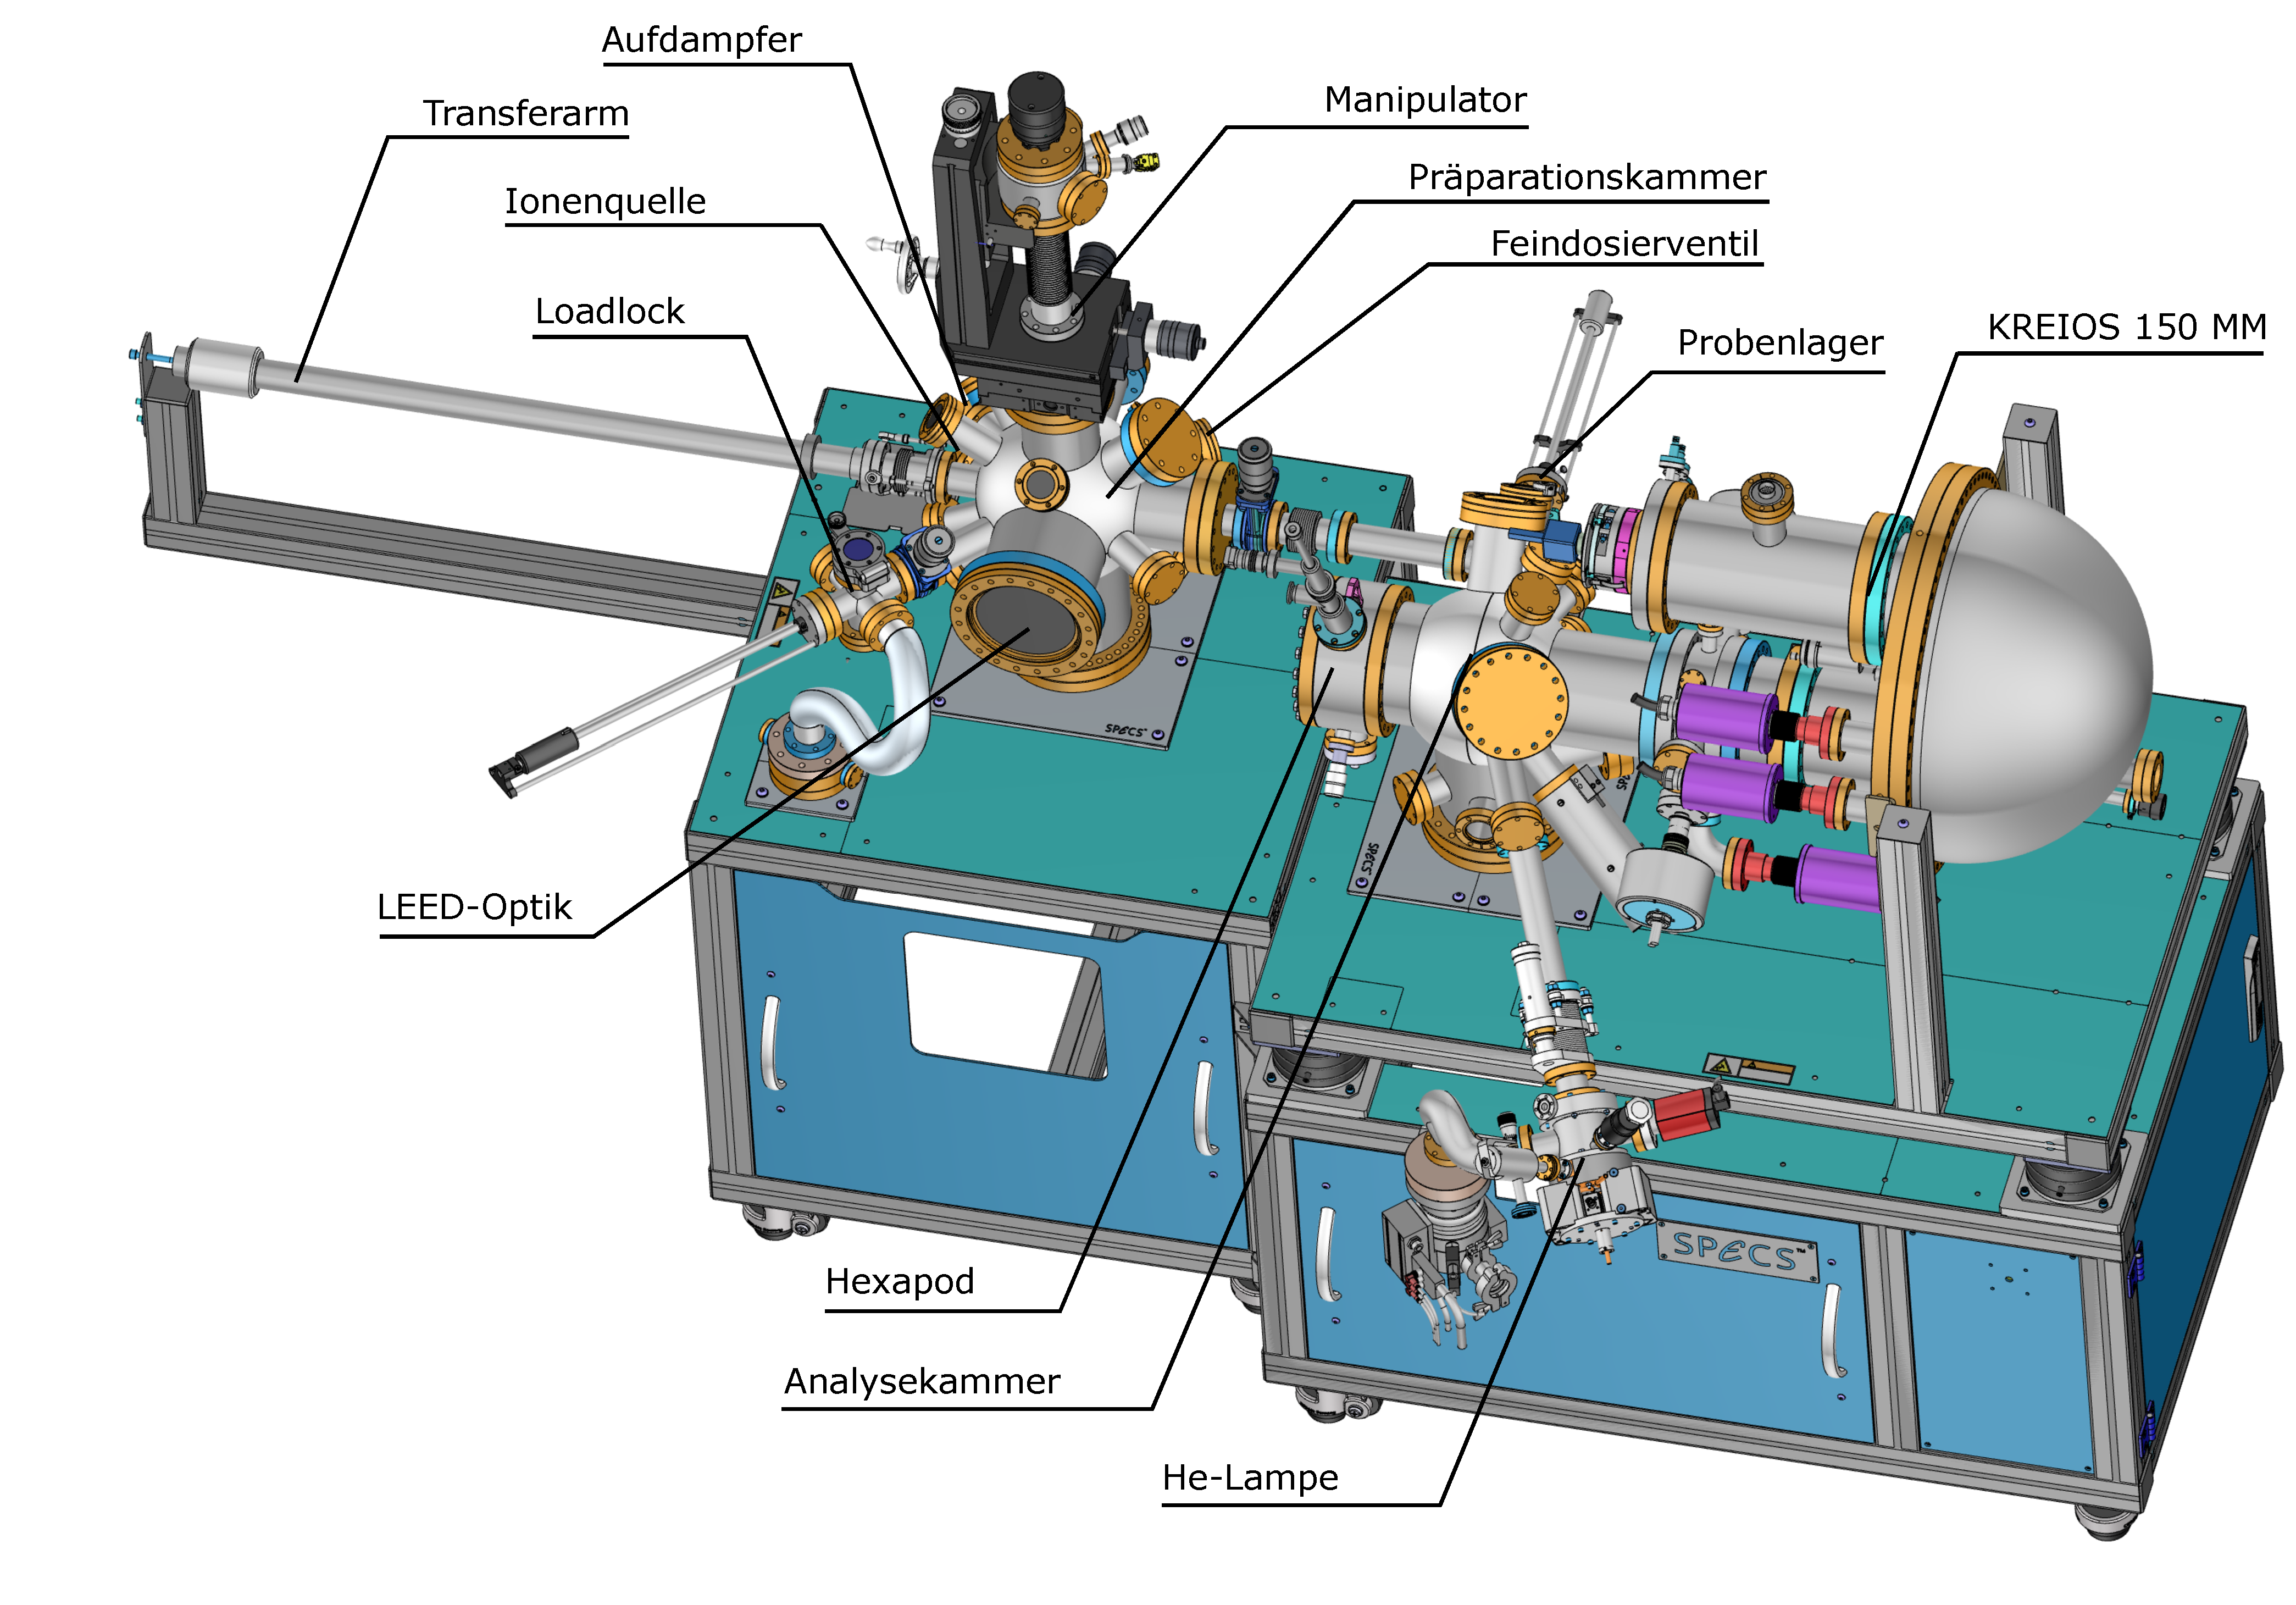
\includegraphics[width=\textwidth]{MM2.pdf}
            \caption{Der für die durchgeführten Experimente verwendete Aufbau.
            Links die Präparationskammer mit Manipulator (Elektronenstoßheizung, Quarzkristallwaage), Aufdampfern, LEED-Optik und Leckventil.
            Rechts die Analysekammer mit der Probenlagerung und dem KREIOS 150 MM.}
            \label{fig:aufbau}
        \end{figure}
        Zur Präparation und Untersuchung der beschriebenen Proben wird der Versuchsaufbau aus \autoref{fig:aufbau} verwendet.
        Dieser besteht aus einer Präparationskammer (links im Bild) und dem Photoelektronenemissionsmikroskop KREIOS 150MM von SPECS (rechts im Bild).
        Beide Kammern sind dabei eigenständige Systeme und werden nur für den Probentransfer verbunden.
        Da es keine Pumpe gibt, die direkt vom Atmosphärendruck bis in den UHV Bereichen kleiner \SI{1e-9}{\milli\bar} reicht, ist ein mehrstufiges Pumpsystem unabdingbar \cite{Henzler}.
        In dem vorliegenden Aufbau wird dies durch Turbomolekularpumpen mit vorgeschalteten Scrollpumpen realisiert.
        Ferner werden diese durch eine Titansublimationspumpe, sowie Ionenpumpe unterstützt.

        In der Präparationskammer befinden sich die Geräte und Komponenten zur Probenpräparation, sowie zur Überprüfung der Oberflächenbeschaffenheit.
        Für die Reinigung der Probe steht eine Ionenquelle zur Verfügung, um die Probe mittels ioneninduzierter Zerstäubung zu reinigen.
        Auf dem Manipulator, mit dem die Probe im Ultrahochvakuum verfahren werden können, ist eine Elektronenstoßheizung montiert, um die Probe aufzuheizen.
        Die Präparationskammer ist mit einer LEED-Optik ausgestattet, wodurch die Oberflächenbeschaffenheit kontrolliert werden kann.
        Desweiteren befindet sich ein Feindosierventil für Sauerstoff, sowie Molekül- und Metallaufdampfer an der Kammer.
        Um die Aufdampfraten der Materialien zu bestimmen, steht eine Quarzkristallwaage am Manipulator zur Verfügung.

        Der KREIOS lässt sich im Realraum als Elektronenmikroskop und im Impulsraum als Impulsmikroskop betreiben.
        Für die vorliegende Arbeit wird dieser allerdings nur im Impulsraum betrieben.
        Vor der Extraktorlinse des Photoelektronenemissionsmikroskopes befindet sich eine 6-Achsen-Piezostage (Hexapod), mit der die Probe in Position gebracht und ausgerichtet werden kann.
        Messungen erfordern eine exakte Ausrichtung der Oberflächennormalen parallel zur Linsenachse und darüber hinaus einen Abstand von \SI{4}{\milli\meter} zum Extraktor~\cite{SPECS-MM}.
        Mit dieser Positioniereinheit kann die Probe auf unter \SI{10}{\kelvin} abgekühlt werden.
        Das Extraktorfeld kann bis auf \SI{29}{\kilo\volt} erhöht werden.
        Als Photonenquelle steht eine Helium-Gasentladungslampe bereit, welche größtenteils Photonen der He-I-Linie (\SI{21.22}{\electronvolt}) emittiert.
        Sie enthält ebenfalls einen kleinen Anteil der He-II-Linie, wodurch es sich um nicht monochromatische Strahlung handelt~\cite{UVS}.
